
\subsection{Pneumothorax Dataset}
\label{subsec:resultPneumothorax}
\subsubsection{Structural Similarity Index Measure}
\label{subsec:ssim}
Figure \ref{fig:ssim} presents a comparison of SSIM scores for various explanation methods on the Pneumothorax dataset \ref{subsubsec:pneumothorax}. These scores were obtained by averaging the results over the test dataset for each pair of saliency map explanations. The computation of the SSIM score involves using the magnitude of the saliency maps, which is normalized to the range of $[0, 1]$.

The results show that the Guided Backpropagation and Guided GradCAM methods produce the most similar saliency maps among all method pairs. Both methods exhibit high similarity on both InceptionV3 and ResNet classifiers, with scores of 0.99 and 0.92, respectively.

Overall, the difference in SSIM scores between the two black boxes indicates that the inner architecture of the black box to some extent influences the appearance of the output explanations. Most of the scores are lower in ResNet, particularly the pairs Saliency--Guided Backpropagation and Saliency--Guided GradCAM, which show a stark difference in SSIM scores (0.71 and 0.72 reductions, respectively). Occlusion consistently shows lower similarity compared to other pairs for both black boxes because there is a difference in the granularity of the explanations produced by Occlusion and other methods. Figure \ref{fig:shapeComparison} provides a comparison of the shapes of various saliency maps, where the saliency maps produced by Occlusion attribute in windows of pixels, while other saliency maps attribute down to the level of each pixel.

\begin{figure}[t]
    \centering
    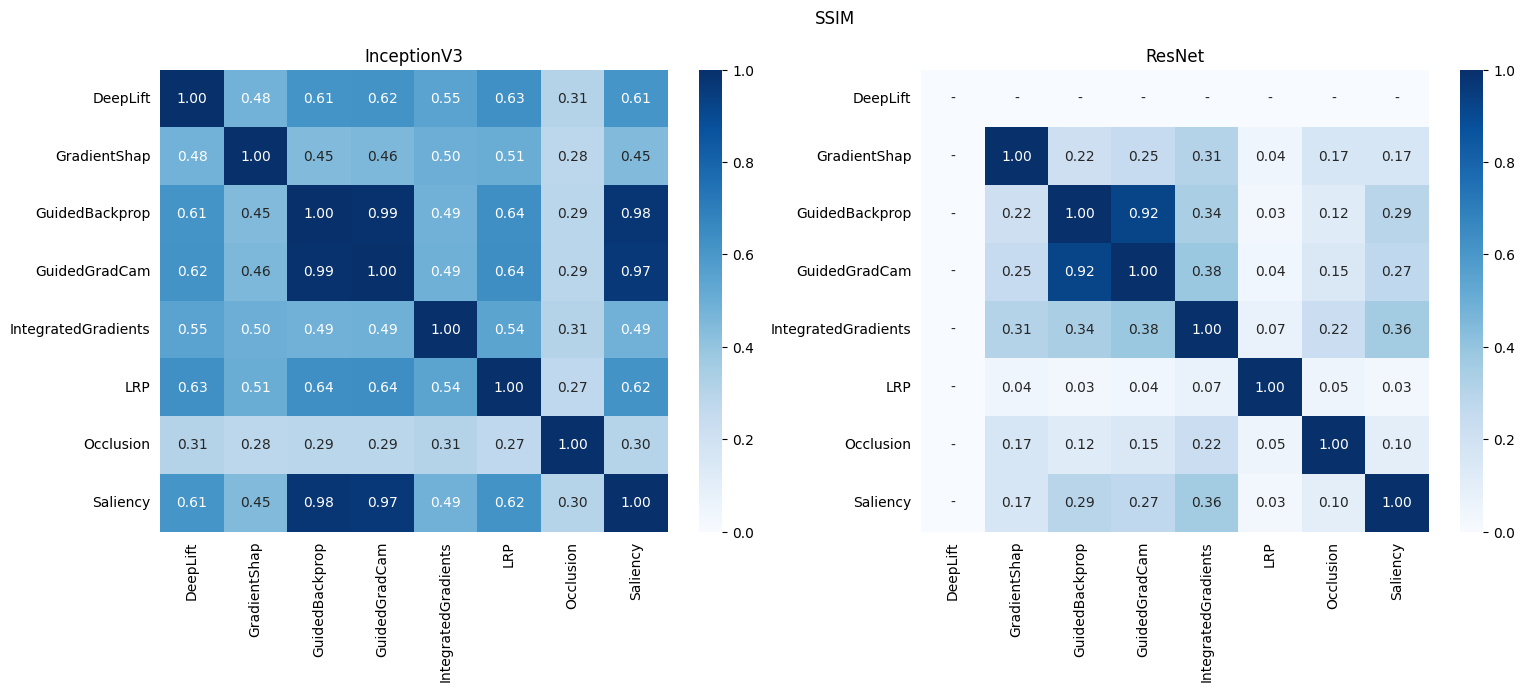
\includegraphics[width=\textwidth]{images/results/pneumothorax/ssim.png}
    \caption{Pairwise structural similarity indices (SSIM) between explanation methods generating for both black boxes (InceptionV3 and ResNet-101). The SSIM scores are computed using the average score over test set data points. Darker colors imply greater similarity in the structure of the two explanations.}
    \label{fig:ssim}
\end{figure}

% TODO: Visualize the input image and the masked region too
\begin{figure}[t]
    \centering
    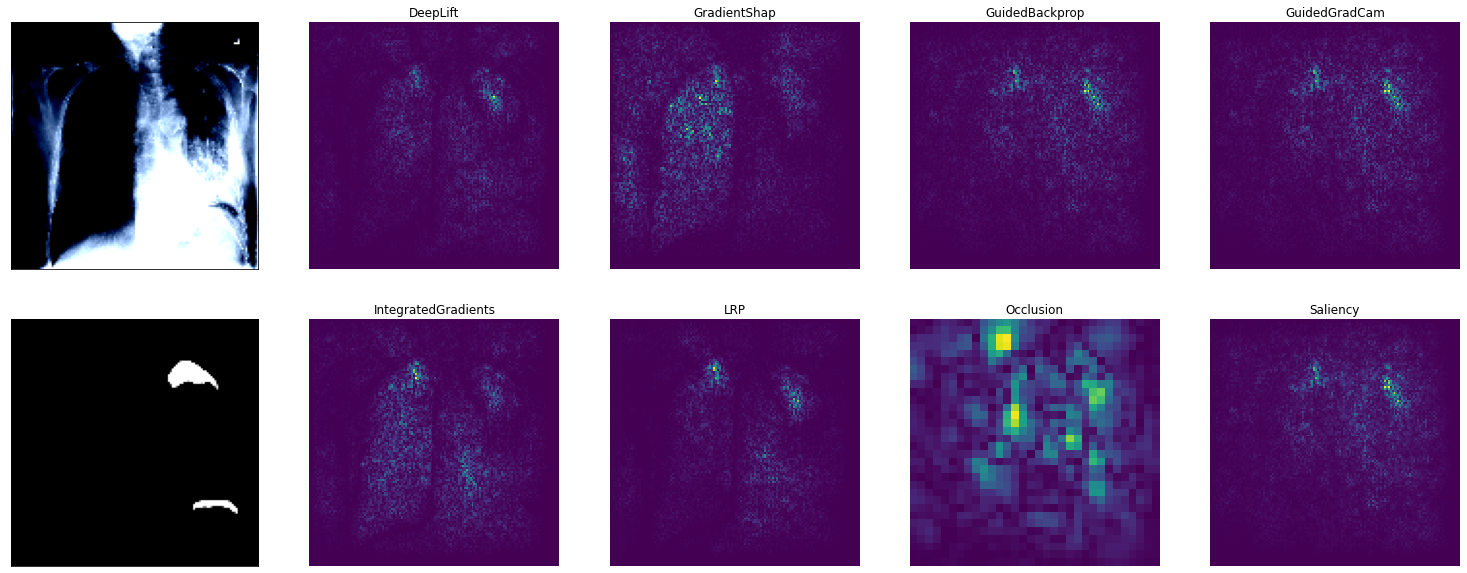
\includegraphics[width=\textwidth]{images/results/shape-comparison-inceptionv3.png}
    \caption{Comparison of the saliency maps generated by the experimental methods with respect to InceptionV3 prediction. Lighter colors indicate more salient pixels.}
    \label{fig:shapeComparison}
\end{figure}

\subsubsection{Feature Agreement}
\label{subsec:featureAgreement}
Figure \ref{fig:featureAgreement} depicts the disagreement between different experiment explanation methods with varying top-$k$ values. The experiments reveal that there is a varying degree of disagreement, but the pair Guided Backpropagation--Guided GradCAM exhibits consistent agreement with each other. Additionally, as $k$ increases, the degree of agreement tends to increase as well.

For InceptionV3, we generally observe that methods with structurally similar saliency maps produce agreeable explanations, while non-structurally similar methods produce higher disagreement. However, this pattern is not consistent when evaluating on ResNet. The agreement scores of LRP with Guided GradCAM and Guided Backpropagation are significantly lower, despite their similar structure. Moreover, the pairs between LRP and Saliency, respectively, with Guided Backpropagation and Guided GradCAM show the highest reduction in agreement scores. With k = 1638, for Saliency, the agreement scores with Guided Backpropagation and Guided GradCAM decrease from 0.92 and 0.91 to 0.36 and 0.38, respectively, with InceptionV3 and ResNet-101. In the case of LRP, the scores are both 0.55 on the two black boxes, down to 0.12 both, respectively.

\begin{figure}[p]
    \centering
    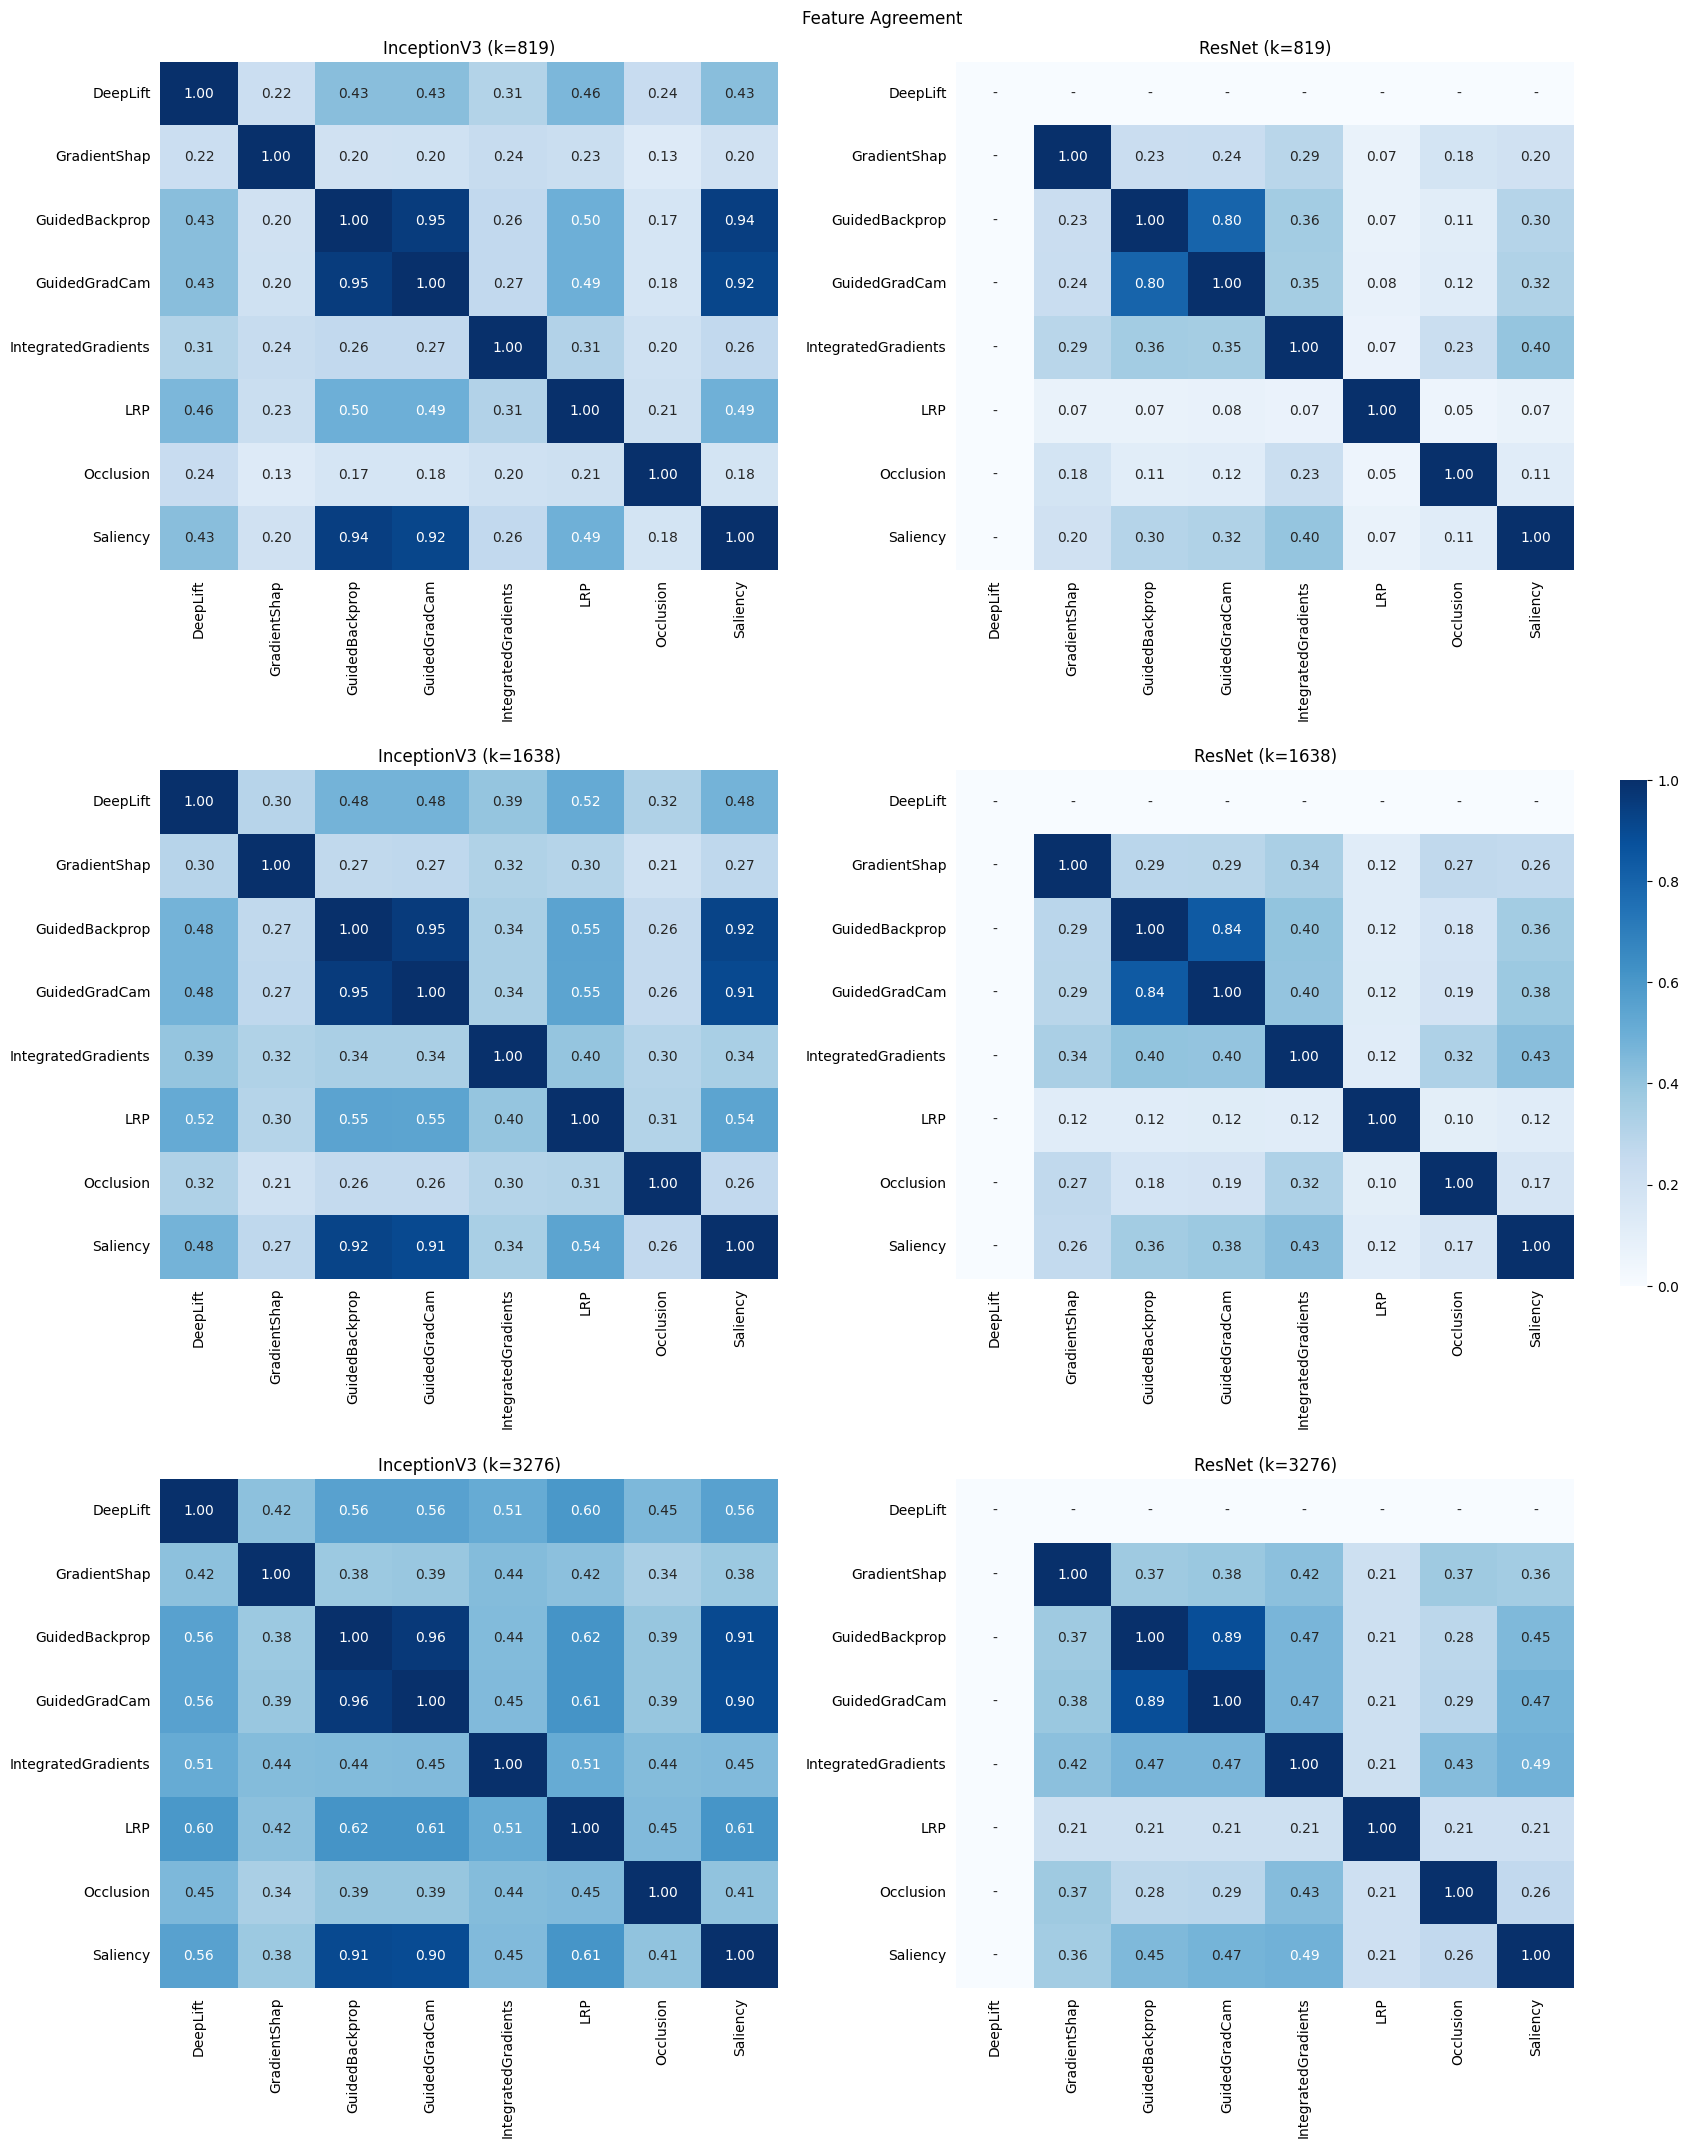
\includegraphics[width=\textwidth]{images/results/pneumothorax/fa.png}
    \caption{Feature agreement between different methods with varying top-$k$ value.}
    \label{fig:featureAgreement}
\end{figure}

\subsection{Sign Agreement}
\label{subsec:signAgreement}
\begin{figure}[t]
    \centering
    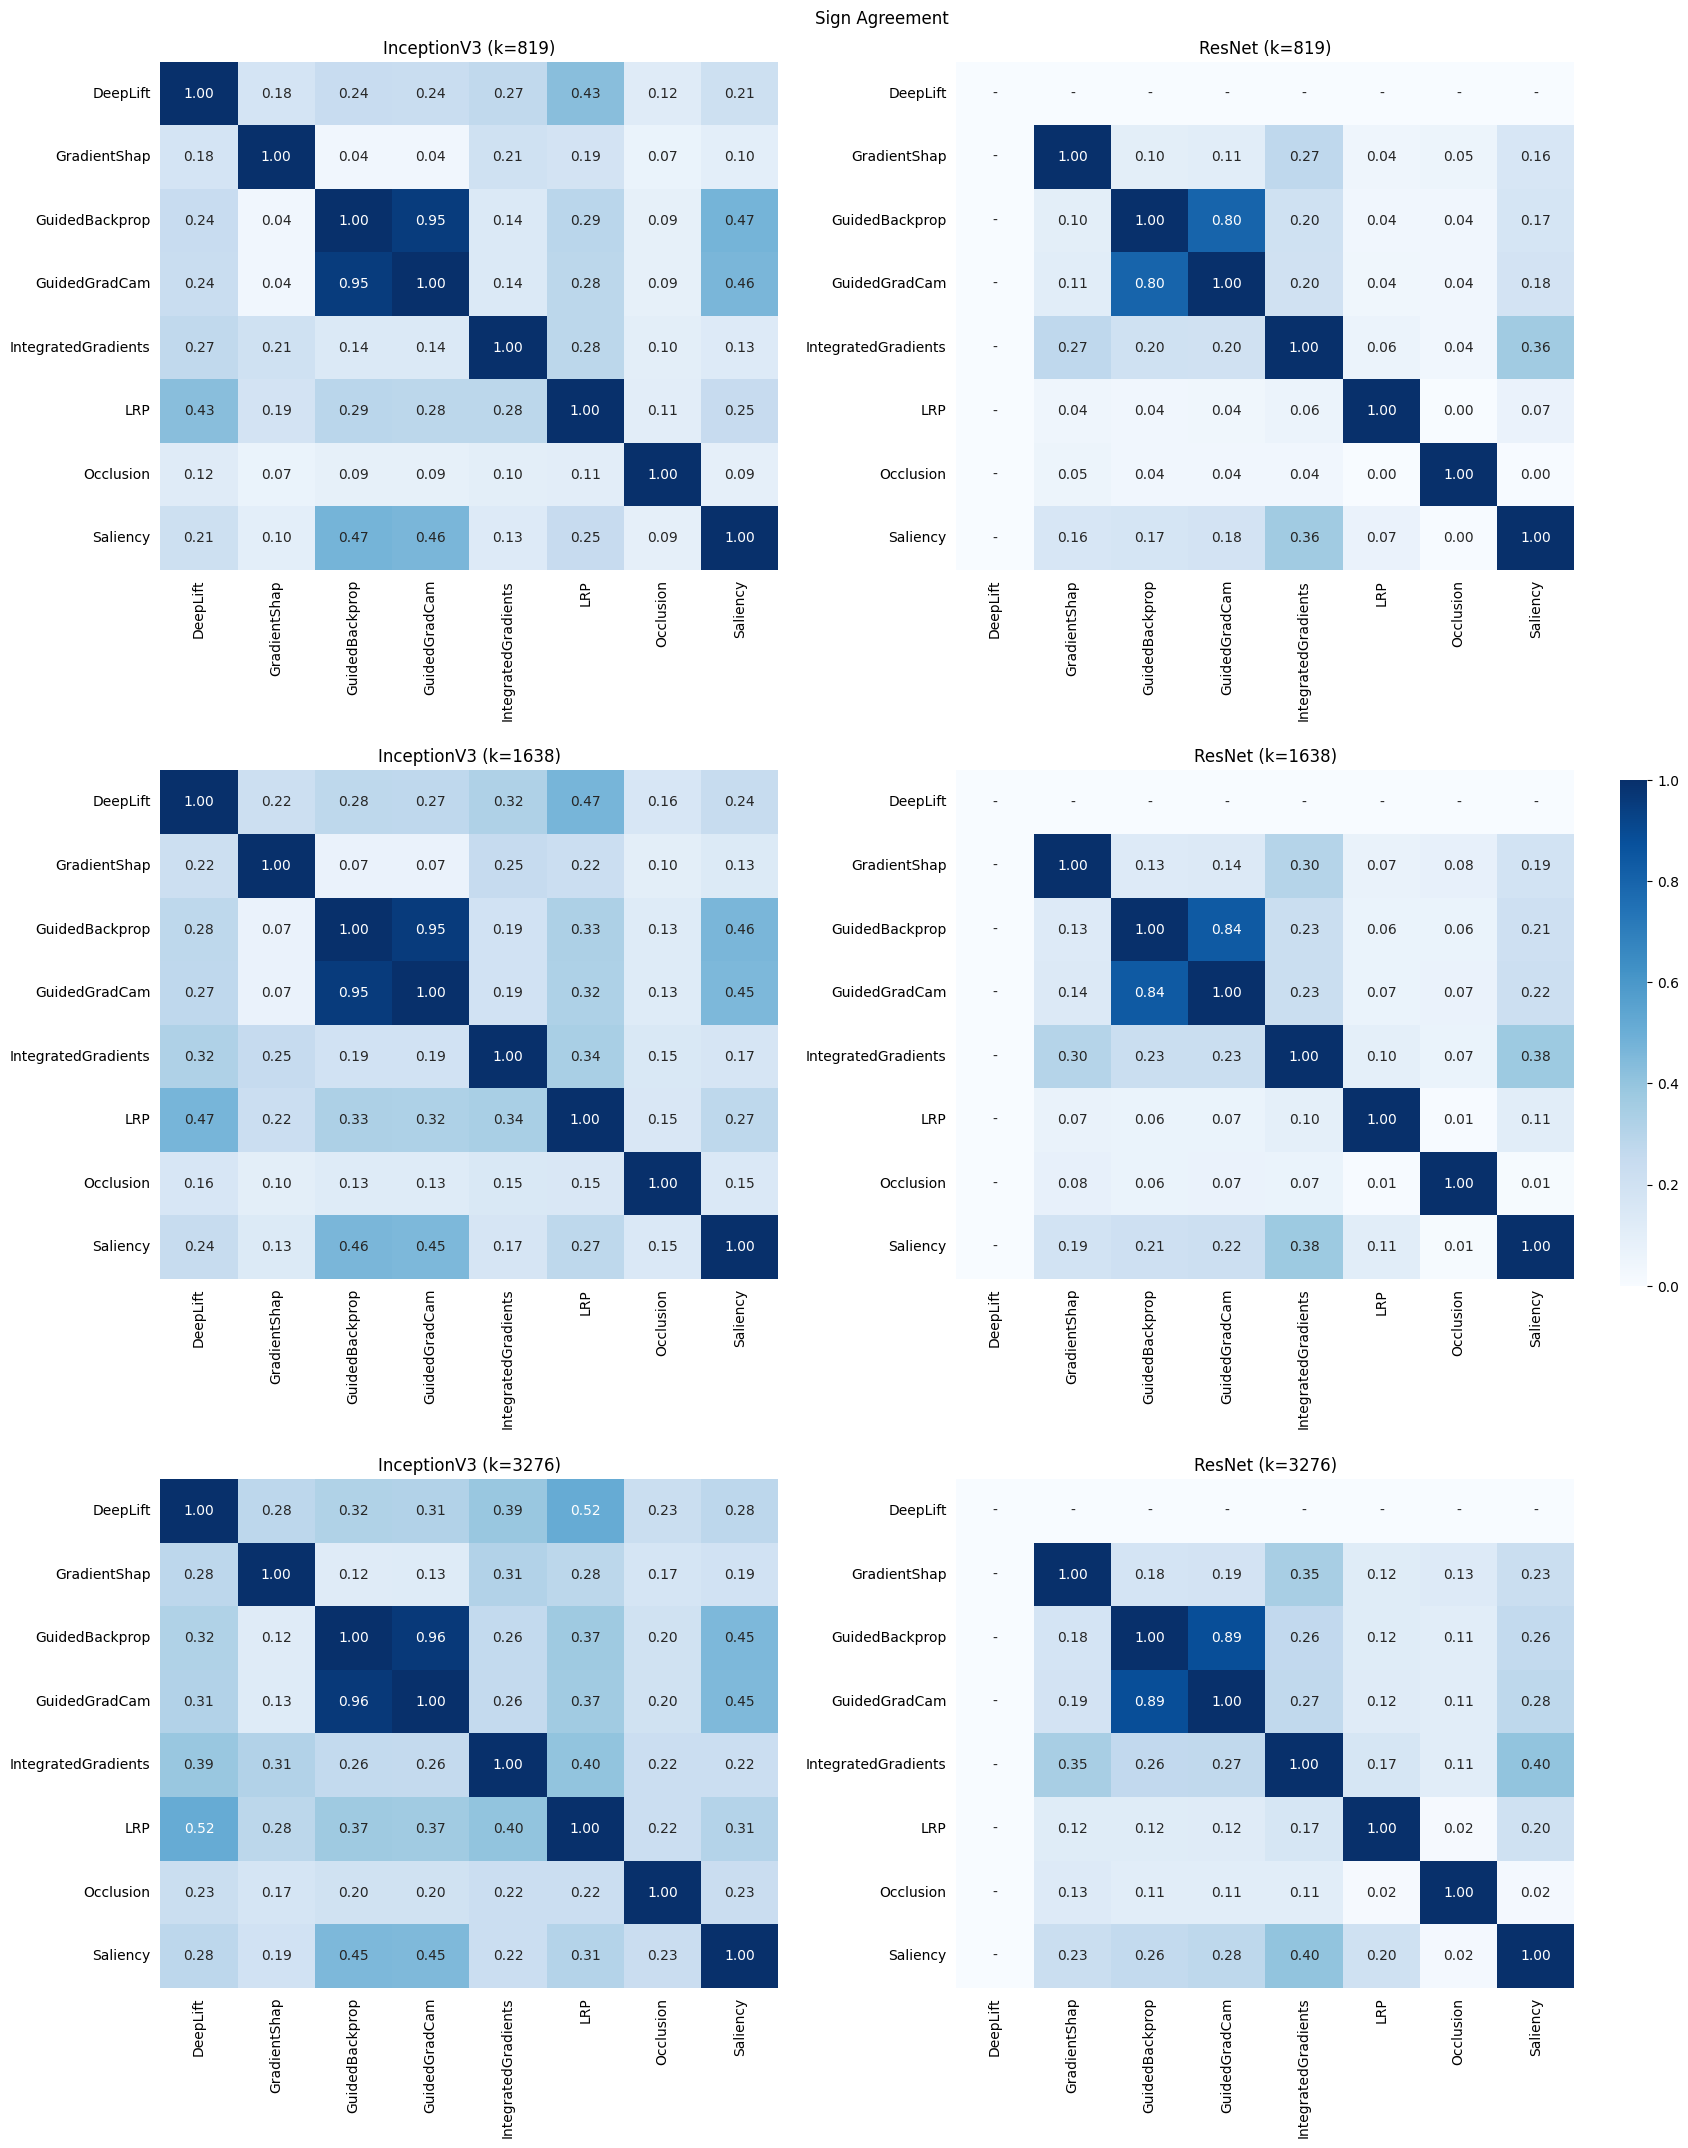
\includegraphics[width=\textwidth]{images/results/pneumothorax/sa.png}
    \caption{Sign agreement between different methods.}
    \label{fig:signAgreement}
\end{figure}

As the conditions become more stringent, the amount of disagreement tends to increase. Figure \ref{fig:signAgreement} displays the average sign agreement score for pairs of explanation methods. Although the agreement scores for pairs that exhibit high agreement in feature agreement (such as Guided Backprop--Guided GradCAM, Saliency--Integrated Gradients, etc.) decrease, they are still significant compared to other pairs. Many pairs demonstrate very low agreement, with scores lower than 0.1.

\begin{figure}
    \centering
    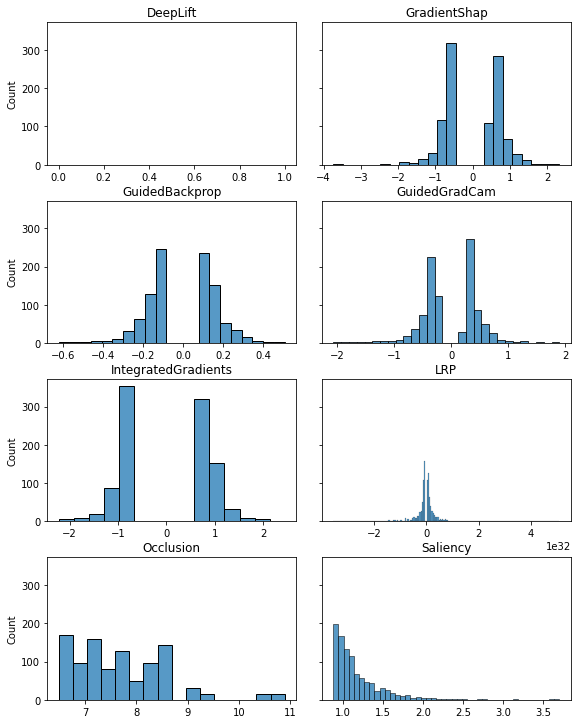
\includegraphics[width=\textwidth]{images/results/saliency-maps-value-distribution-resnet.png}
    \caption{The distributions of the saliency map values (within the top-$k$ magnitude) produced by the explanation methods, evaluating on ResNet model.}
    \label{fig:saliencyMapsValueDistributionResnet}
\end{figure}

\begin{figure}
    \centering
    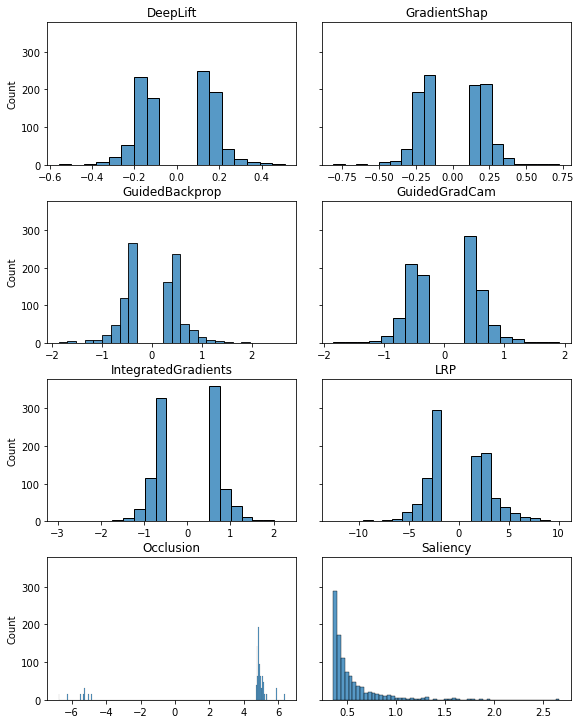
\includegraphics[width=\textwidth]{images/results/saliency-maps-value-distribution-inceptionv3.png}
    \caption{The distributions of the saliency map values (within the top-$k$ magnitude) produced by the explanation methods, evaluating on InceptionV3 model.}
    \label{fig:saliencyMapsValueDistributionInceptionV3}
\end{figure}

An interesting observation from this result is that most of the sign agreement scores for all pairs are approximately half of the corresponding feature agreement scores in both black boxes. This is because most explanation methods (with the exception of Occlusion and Saliency) generate saliency maps with the distribution of the attribution scores having a mean near 0. Figures \ref{fig:saliencyMapsValueDistributionResnet} and \ref{fig:saliencyMapsValueDistributionInceptionV3} illustrate that all gradient-based methods distribute negative and positive values similarly among the most important pixels.

This suggests that the metric sign agreement may not provide useful information when used as a disagreement measure for saliency maps. However, our observations do not negate the potential use of this metric for other types of explanations. We urge further research on different types of explanation methods to confirm its usefulness.

\subsubsection{Rank Correlation}
\label{subsec:rankCorrelation}

\begin{figure}
    \centering
    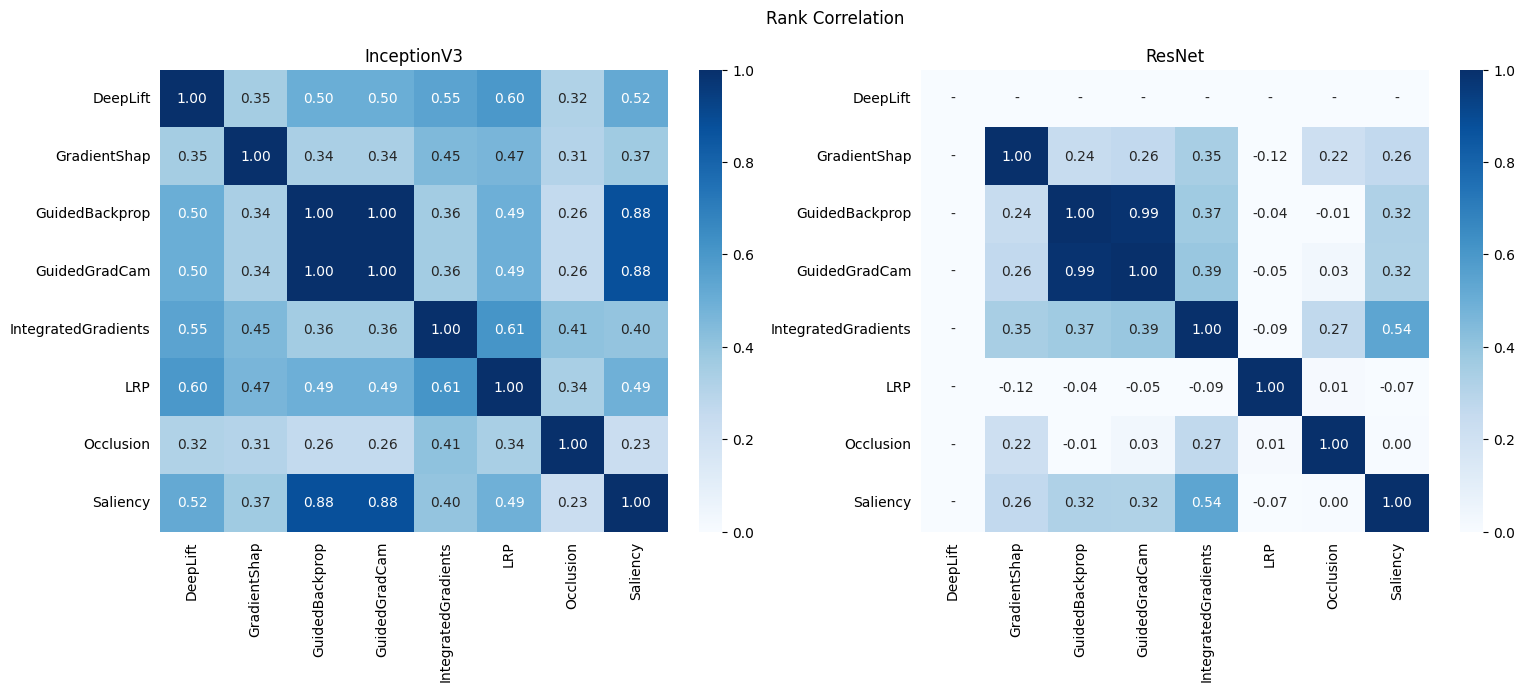
\includegraphics[width=\textwidth]{images/results/pneumothorax/rc.png}
    \caption{Rank correlation between different methods}
    \label{fig:rankCorrelation}
\end{figure}
This section we present the disagreement scores between explanation methods when using the metric rank correlation. The scores are summarized in figure \ref{fig:rankCorrelation} and are computed on instances where pneumothorax masks are available (i.e., instances where the ground-truth label is has-pneumothorax). Computing the rank correlation score with respect to the ground-truth masks provides insight into how agreeable the explanation methods are in considering the relative importance of pixels in the ground-truth area. In simpler terms, the metric indicates whether two saliency maps consistently consider the importance ranking of pixels in the actual pneumothorax area for the black box's decision.

The results show that highly agreeable pairs, as shown in previous experiments, remain consistent with each other in rank correlation, while pairs that strongly disagree with each other also remain that way.
